\documentclass[11pt]{article}

\usepackage[utf8]{inputenc}
\usepackage[T1]{fontenc}
\usepackage{lmodern}
\usepackage{microtype}
\usepackage[margin=0.82in,headheight=14pt]{geometry}
\usepackage{amsmath,amssymb}
\usepackage{booktabs,longtable,tabularx,array,multirow}
\usepackage{graphicx}
\usepackage{tikz}
\usetikzlibrary{arrows.meta,positioning,fit,calc}
\usepackage{xcolor}
\usepackage{enumitem}
\usepackage{listings}
\usepackage{float}
\usepackage{caption}
\usepackage{fancyhdr}
\usepackage{titlesec}
\usepackage{mdframed}
\usepackage[numbers,sort&compress]{natbib}
\usepackage[hidelinks]{hyperref}
\usepackage{bookmark}

\definecolor{Ink}{HTML}{000000}
\definecolor{Navy}{HTML}{17324D}
\definecolor{Blue}{HTML}{0072B2}
\definecolor{Orange}{HTML}{E69F00}
\definecolor{BluishGreen}{HTML}{009E73}
\definecolor{Vermillion}{HTML}{D55E00}
\definecolor{Slate}{HTML}{5F6B73}
\definecolor{LightGray}{HTML}{E6E6E6}
\definecolor{PanelGray}{HTML}{F1F1F1}
\definecolor{PaleBlue}{HTML}{EEF5FA}
\definecolor{PaleTeal}{HTML}{EDF8F5}
\definecolor{PaleOrange}{HTML}{FFF7E8}
\definecolor{PaleGray}{HTML}{F4F6F7}

\hypersetup{
  colorlinks=true,
  unicode=true,
  pdfencoding=auto,
  pdflang={en-US},
  pdfdisplaydoctitle=true,
  linkcolor=Ink,
  citecolor=Ink,
  urlcolor=Ink,
  pdftitle={Event-Driven L2 Replay},
  pdfauthor={Pranav Pillai},
  pdfsubject={BTCUSDT passive market-making research and execution simulation},
  pdfkeywords={market microstructure, limit order book, market making, OFI, replay}
}

\setlist[itemize]{leftmargin=1.45em,itemsep=0.25em,topsep=0.35em}
\setlist[enumerate]{leftmargin=1.55em,itemsep=0.25em,topsep=0.35em}
\renewcommand{\arraystretch}{1.18}
\newcolumntype{Y}{>{\raggedright\arraybackslash}X}
\newcolumntype{R}{>{\raggedleft\arraybackslash}X}
\newcolumntype{L}[1]{>{\raggedright\arraybackslash}p{#1}}

\titleformat{\section}{\Large\bfseries\color{Ink}}{\thesection}{0.7em}{}
\titleformat{\subsection}{\large\bfseries\color{Ink}}{\thesubsection}{0.6em}{}
\titleformat{\subsubsection}{\normalsize\bfseries\color{Ink}}{\thesubsubsection}{0.55em}{}
\titlespacing*{\section}{0pt}{2.1ex plus 0.8ex}{0.9ex}
\titlespacing*{\subsection}{0pt}{1.7ex plus 0.5ex}{0.55ex}

\pagestyle{fancy}
\fancyhf{}
\lhead{\small\color{Ink}L2 Market Microstructure System}
\rhead{\small\color{Ink}Pranav Pillai}
\cfoot{\small\color{Ink}\thepage}
\renewcommand{\headrulewidth}{0.3pt}

\newmdenv[
  backgroundcolor=PanelGray,
  linecolor=Ink,
  linewidth=0.8pt,
  roundcorner=3pt,
  skipabove=0.8em,
  skipbelow=0.8em,
  innerleftmargin=10pt,
  innerrightmargin=10pt,
  innertopmargin=8pt,
  innerbottommargin=8pt
]{statusbox}

\newmdenv[
  backgroundcolor=LightGray,
  linecolor=Ink,
  linewidth=0.8pt,
  roundcorner=3pt,
  skipabove=0.8em,
  skipbelow=0.8em,
  innerleftmargin=10pt,
  innerrightmargin=10pt,
  innertopmargin=8pt,
  innerbottommargin=8pt
]{cautionbox}

\lstdefinestyle{projectcode}{
  basicstyle=\ttfamily\small,
  backgroundcolor=\color{PaleGray},
  frame=single,
  rulecolor=\color{PaleGray},
  breaklines=true,
  columns=fullflexible,
  keepspaces=true,
  showstringspaces=false,
  xleftmargin=0.5em,
  xrightmargin=0.5em,
  aboveskip=0.7em,
  belowskip=0.7em
}

\newcommand{\code}[1]{\texttt{\detokenize{#1}}}
\newcommand{\repo}{\href{https://github.com/pranavpillaiNUS/l2-mm-system}{github.com/pranavpillaiNUS/l2-mm-system}}
\newcommand{\artifact}[1]{\href{https://github.com/pranavpillaiNUS/l2-mm-system/blob/main/#1}{\nolinkurl{#1}}}
\newcommand{\directory}[1]{\href{https://github.com/pranavpillaiNUS/l2-mm-system/tree/main/#1}{\nolinkurl{#1}}}
\newcommand{\frozenartifact}[1]{\href{https://github.com/pranavpillaiNUS/l2-mm-system/blob/106695026ca64ae232f07103ae380b49c2a4d49f/#1}{\nolinkurl{#1}}}
\newcommand{\ReportVersion}{0.1}
\newcommand{\ReportDate}{4 August 2026}
\newcommand{\LegacyModel}{\code{legacy_book_update_v1}}
\newcommand{\CurrentModel}{\code{event_driven_v2}}

% Generated by scripts/build_report_assets.py; do not edit by hand.
\newcommand{\PhaseAQcZeroMean}{-0.686}
\newcommand{\PhaseAQcZeroLow}{-1.883}
\newcommand{\PhaseAQcZeroHigh}{+0.290}
\newcommand{\PhaseAQcOneMean}{-1.043}
\newcommand{\PhaseAQcOneLow}{-2.332}
\newcommand{\PhaseAQcOneHigh}{-0.032}
\newcommand{\OFITStat}{64.63}
\newcommand{\OFIRSquared}{0.0366}
\newcommand{\OFIEffect}{+0.123}
\newcommand{\OFIConditionalQcZero}{-0.376}
\newcommand{\OFIConditionalQcOne}{+0.127}
\newcommand{\OFIMinCountQcZero}{154}
\newcommand{\OFIMinCountQcOne}{201}
\newcommand{\QueueMatchedQcZero}{-9.75}
\newcommand{\QueueMatchedQcOne}{-23.65}
\newcommand{\MatchedBreakEvenQcZero}{1.351}
\newcommand{\MatchedBreakEvenQcOne}{0.426}
\newcommand{\FullRebateQcZero}{0.769}
\newcommand{\FullRebateQcOne}{1.351}
\newcommand{\SnapshotReceiptMedianMs}{250.5}
\newcommand{\SnapshotReceiptPninetyMs}{672.9}
\newcommand{\SnapshotReceiptMaxMs}{2,335}
\newcommand{\SnapshotBridgeMedianMs}{150.0}
\newcommand{\SnapshotPreBridgeFillsQcZero}{2}
\newcommand{\SnapshotPreBridgeFillsQcOne}{4}
\newcommand{\DevelopmentWindows}{24}
\newcommand{\HoldoutWindows}{12}
\newcommand{\ManifestHours}{1193}
\newcommand{\ManifestValidHours}{775}
\newcommand{\ManifestInvalidHours}{418}
\newcommand{\ManifestHashShort}{a3a99b0a616a}
\newcommand{\PanelHashShort}{760c55b7c092}


\begin{document}
\hypersetup{pageanchor=false}

\begin{titlepage}
  \thispagestyle{empty}
  \vspace*{0.8cm}
  \noindent{\color{Ink}\rule{\textwidth}{1.8pt}}
  \vspace{0.8cm}

  {\Huge\bfseries\color{Ink} Event-Driven L2 Replay\par}
  \vspace{0.45cm}
  {\Large An artifact-verifiable BTCUSDT market-making case study\par}

  \vspace{1.1cm}
  {\large Pranav Pillai\par}
  \vspace{0.2cm}
  {\normalsize Report version \ReportVersion\quad--\quad\ReportDate\par}
  {\small Frozen research snapshot: \code{1066950}\par}
  \vspace{0.15cm}
  {\normalsize Repository: \repo\par}

  \vspace{1.0cm}
  \begin{statusbox}
    \textbf{Scope in one sentence.} This repository is a tested Python research
    system for deterministic limit-order-book reconstruction, event-driven
    execution simulation, and hypothesis testing. It makes no claim of a
    profitable live strategy or exchange-validated production execution.
  \end{statusbox}

  \vspace{0.5cm}
  \textbf{Central finding.} In the frozen 24-window development study,
  normalized order-flow imbalance was strongly associated with one-second
  forward mid-price movement at the population level (HAC
  $t=\OFITStat$, effect $\OFIEffect$ bps per signal standard deviation), but
  the pre-specified fill-conditioned screen failed at both queue-model
  endpoints. The conditional bucket pattern was non-monotone, so the proposed
  OFI-gated maker was not advanced and no candidate strategy was evaluated on
  the holdout.

  \vspace{0.55cm}
  \begin{cautionbox}
    \textbf{Model-version boundary.} All economic numbers in this report are
    frozen historical evidence produced by \LegacyModel. The current Python
    behavioral reference, \CurrentModel, has passed implementation acceptance but its
    development-panel economic rerun is pending. The old and current models are
    deliberately not conflated.
  \end{cautionbox}

  \vfill
  {\small\color{Ink}
    Venue and instrument: Binance spot BTCUSDT. L2 research period: April--May
    2026. Software: Python 3.11. The raw capture is not distributed, canonical
    derived artifacts and integrity identities are committed.
  }
  \vspace{0.4cm}
  \noindent{\color{Ink}\rule{\textwidth}{1.8pt}}
\end{titlepage}

\hypersetup{pageanchor=true}
\pagenumbering{roman}
\begin{abstract}
This report documents the design, failure analysis, and present state of a
market-microstructure research system. The system records Binance spot depth
and trades, reconstructs the L2 book with decimal arithmetic, merges events
deterministically, simulates post-only passive orders with modeled queue
position and latency, and produces auditable P\&L, markout, queue, and signal
diagnostics. An earlier hourly bar backtester established reusable interfaces
but is retained only as an educational precursor because its same-close
execution and return annualization are too coarse for rigorous strategy
evidence.

The frozen development study used 24 non-overlapping five-hour windows and two
endpoints for queue cancellation credit. The passive microprice baseline did not
demonstrate stable positive economics. Normalized one-second OFI had a strong,
monotone population association with forward mid drift, but its pre-specified
conditional comparison was only \OFIConditionalQcOne\ bps under proportional
credit and \OFIConditionalQcZero\ bps under no credit, below a 1.0 bps screening
threshold. Because the full conditional dose-response was non-monotone, the
evidence did not justify advancing the candidate. No candidate strategy was
evaluated on the 12-window holdout. Only its pre-strategy regime descriptors
were examined.

A subsequent audit found that the historical simulator quantized private order
arrival to book updates and applied cancels immediately. Rather than relabel the
old results, the project froze them under \LegacyModel\ and built
\CurrentModel, with exact scheduling on the model's millisecond clock,
post-response-gated snapshot recovery, cancel/fill races, own-order FIFO,
trade-volume conservation, fail-closed gaps, and a hard working-exposure
envelope. At the 4 August 2026 publication checkpoint, a fresh clone reports
376 deterministic tests passed and three optional raw-data smoke checks skipped
under Python 3.11. All 379 pass when the selected captures are restored. The live
recorder check is a separate manual network operation. Economic results under
the current model remain pending. The project contribution is therefore the combination of a transparent
negative/conditional development result, explicit model-risk boundaries, and
an artifact-verifiable Python behavioral reference for later performance work.
\end{abstract}

\tableofcontents
\clearpage
\pagenumbering{arabic}

\section{Executive Summary}

\subsection{Research question}

The project asks a narrower question than ``can an order-book signal predict
the next price move?'' It asks whether a signal remains useful after the
strategy's own execution process selects which observations become passive
fills. That distinction is central to market making. A resting limit order is
most likely to trade when an aggressor reaches it, and that event can be
informative about the next move. A population-level forecast can therefore be
real while the subset of states in which the maker is filled remains toxic.
This is the adverse-selection problem described in classical microstructure
models such as \citet{glosten1985}, and OFI is motivated by the empirical link
between order-book events and short-horizon price impact in
\citet{cont2014}.

The system was built to measure that gap between \emph{signal association} and
\emph{execution-conditioned economics} without hiding assumptions about queue
position, event ordering, fees, or missing data.

\subsection{What was built}

The current repository contains four connected capabilities:

\begin{itemize}
  \item a bar-level backtesting scaffold retained as project history,
  \item spot and perpetual-futures data recorders, with spot L2 and trade data
        forming the completed research dataset,
  \item a deterministic event replay and execution simulator with post-only
        behavior, configurable latency, partial fills, L2-derived FIFO queue
        position, and maker/taker fee assignment, and
  \item a research pipeline for integrity screening, panel selection,
        bootstrap intervals, OFI diagnostics, model stress, decision gates,
        artifact hashing, and a strategy-sealed holdout.
\end{itemize}

The most important engineering work occurred after the historical study. Model
audits showed that the old simulator activated private orders only on the next
book update, made cancellations immediate, and applied REST snapshot state at a
local tag captured before the request completed. The current \CurrentModel\
implementation instead schedules order and cancel arrivals on the replay clock,
gates legacy snapshot recovery on a post-response receipt proxy, models
cancel/fill races, conserves recorded trade volume across overlapping own
orders, and refuses to write into the frozen result root.

\subsection{Evidence and decision}

The frozen development experiment covers \DevelopmentWindows\ non-overlapping
five-hour windows. The passive microprice baseline was negative in 18 of 24
windows at each tested queue endpoint. The proportional-credit mean was
\PhaseAQcOneMean\ USDT per window with a 95\% window-bootstrap interval
$[\PhaseAQcOneLow,\PhaseAQcOneHigh]$. The no-credit mean was
\PhaseAQcZeroMean\ with interval
$[\PhaseAQcZeroLow,\PhaseAQcZeroHigh]$.

Normalized OFI was much stronger than microprice as a population signal. At one
second, the pooled association had HAC $t=\OFITStat$, $R^2=\OFIRSquared$, and
an effect of \OFIEffect\ bps per signal standard deviation. All 24 per-window
coefficients were positive, and the six unconditional bucket averages were
monotone.

The pre-specified conditional screen nevertheless failed. It compared the
most-populated adverse side-aligned bucket with the most-populated nonnegative
bucket at a 30-second horizon. The separation was
\OFIConditionalQcOne\ bps under proportional queue credit and
\OFIConditionalQcZero\ bps with no credit, below the 1.0 bps screen. The full
bucket pattern was non-monotone, including a smaller intermediate bucket with a
more favorable mean. Consequently, the correct conclusion is not that OFI is
universally useless after conditioning. It is that the defined conditional
gate did not yield a robust, monotone separation strong enough to justify a
candidate run. The \code{OFIGatedMM} candidate was blocked and no holdout
strategy result was generated.

\subsection{Why the negative result matters}

The project rejected several opportunities to report an attractive but weakly
supported result:

\begin{itemize}
  \item Early apparent profitability contained taker fills created by latency,
        post-only enforcement removed that interpretation.
  \item Snapshot synchronization and stale-diff issues were corrected and the
        affected study was regenerated.
  \item A strong unconditional OFI statistic was not treated as executable edge
        after the fill-conditioned gate failed.
  \item A candidate was not tried on the strategy-sealed holdout after failing its
        development premise.
  \item A later execution-timing flaw created a new model and artifact namespace
        instead of being retroactively attached to old results.
\end{itemize}

For a research record, this audit trail is more informative than a fragile
positive backtest. It demonstrates the ability to define an estimand, identify
where simulation assumptions enter it, reject contaminated evidence, and stop
an experiment when the protocol says to stop.

\subsection{Version map}

The project has similarly named study and model versions. Table
\ref{tab:version-map} is the authoritative map.

\begin{table}[H]
\centering
\caption{Study and execution-model version map.}
\label{tab:version-map}
\begin{tabularx}{\textwidth}{@{}L{0.21\textwidth}L{0.31\textwidth}Y@{}}
\toprule
Label & Meaning & Status and permitted claim \\
\midrule
Study V1 & Six-window exploratory study & Frozen and superseded by the larger historical study. \\
Artifact V2 & 24-window Phase A/B/C development study & Frozen historical evidence, generated at research commit \code{1066950}. \\
Legacy model & Historical private-timing and queue semantics & Superseded, the source of V2 execution-derived numbers. \\
Current model & Current Python behavioral reference & Mechanics accepted locally, no development-panel economics yet. \\
Artifact V3 & Results produced by \CurrentModel & Pending, the development rerun has not been executed. \\
Holdout & 12 selected five-hour windows & Strategy-sealed, no candidate strategy output exists. \\
\bottomrule
\end{tabularx}
\end{table}

\begin{statusbox}
\textbf{Current public interpretation.} The repository is ready to demonstrate
the engineering reference and the discipline of the frozen case study. It is
not yet ready to claim that the historical economic conclusion survives the
current execution model. The V3 development rerun is the next research
milestone.
\end{statusbox}

\section{Project Evolution}

\subsection{Phase 1: an educational backtesting scaffold}

The project began with BTCUSDT hourly OHLCV bars. Four simple strategy families
were implemented behind a common interface: momentum, mean reversion, moving
average crossover, and Bollinger bands. The surrounding framework separated
configuration, data loading, portfolio accounting, transaction costs, metrics,
plotting, parameter sweeps, and walk-forward orchestration.

That phase produced valuable engineering lessons: fees could erase a gross
edge, stateful strategy instances had to be recreated between runs, expanding
window selection changed parameter rankings, and orchestration code required as
much testing as individual components. Those lessons directly informed the L2
design.

The historical Phase 1 performance table is \emph{not} treated as rigorous
strategy evidence in this report. A later publication audit identified four
limitations:

\begin{enumerate}
  \item strategies observe the current bar close and execute at that same close,
  \item hourly equity observations were annualized with 365 periods per year,
  \item the displayed ``OOS Sharpe'' is a mean of monthly Sharpe estimates rather
        than the Sharpe of one stitched OOS return series, and
  \item the historical optimizer source was overwritten by the plotting pass.
        A runner has since been reconstructed from the logged grids, but the
        original performance artifacts are not promoted to current evidence.
\end{enumerate}

The current metrics helper now infers the observation frequency from its
timestamp index, and a regression test covers the hourly-versus-daily scaling.
The historical Phase 1 CSVs were not rewritten, so their published ratios
retain the original limitation.

These issues do not affect the independently implemented L2 replay. They do mean
that Phase 1 should be read as an engineering precursor and a record of learning,
not as evidence that any bar strategy generalizes. This distinction is now made
explicit rather than allowing precise-looking ratios to imply a stronger study.

\subsection{Why bars were insufficient}

Market making depends on phenomena that bars remove:

\begin{itemize}
  \item whether a limit order was passive when it reached the exchange,
  \item volume ahead at a price and how trades advance queue position,
  \item partial fills and residual inventory,
  \item entry and cancellation latency,
  \item event ordering when book changes and trades share a timestamp, and
  \item whether a fill is followed by a favorable or adverse price move.
\end{itemize}

The project therefore shifted from optimizing directional bar signals to
reconstructing a deterministic L2 event path and treating execution as part of
the hypothesis.

\subsection{Phase 2: replay, execution, and a frozen study}

Phase 2 added data recorders, snapshot-aware parsers, an L2 book, depth/trade
merging, execution simulation, passive quoting strategies, and markout/P\&L
analysis. Exploratory work selected a microprice reference, a 2 USDT
half-spread, and a five-second requote interval. Six anchor windows were later
retained inside a larger 24-window development panel. Because those anchors
were involved in exploration, the final panel is broader and pre-selected but
not a wholly untouched confirmation sample. The report preserves that fact.

The expanded study was organized as:

\begin{description}[leftmargin=5.4em,style=nextline]
  \item[Phase A] remeasure the fixed passive baseline at queue-credit endpoints,
  \item[Phase B] test whether OFI satisfies a population and fill-conditioned
        premise gate before running a strategy that uses it, and
  \item[Phase C] stress queue-cancellation credit and entry latency, then close
        the development arc if no candidate qualifies.
\end{description}

No candidate qualified. No candidate strategy was evaluated on the holdout.

\subsection{Phase 2.5: execution-model closure}

After the study was frozen, review of private-event timing found that the
historical engine used the next depth event as the activation point for an order
whose modeled arrival might have occurred earlier. Cancels were immediate, so
cancel/fill races were absent. Overlapping own orders also required a stronger
FIFO decomposition to guarantee that one recorded trade could not fill more
simulated volume than it contained.

The response was a provenance boundary:

\begin{itemize}
  \item historical artifacts were labeled \LegacyModel,
  \item the frozen result directory became write-protected to current scripts,
  \item the new implementation was named \CurrentModel,
  \item current results were assigned a distinct V3 namespace, and
  \item cross-model comparisons were restricted to descriptive sensitivity,
        not treated as estimates from the same execution process.
\end{itemize}

This is the current stage. The Python mechanics are tested, V3 development
economics remain pending.

\subsection{Timeline and decision discipline}

\begin{table}[H]
\centering
\caption{Condensed project timeline.}
\begin{tabularx}{\textwidth}{@{}L{0.15\textwidth}L{0.25\textwidth}Y@{}}
\toprule
Period & Milestone & Research consequence \\
\midrule
Jan--Apr 2026 & Bar framework and walk-forward exercise & Established reusable interfaces and exposed the importance of costs and state isolation. \\
Apr--May 2026 & L2 recorder, replay, execution, and exploratory baseline & Profit contaminated by accidental taker fills was rejected after post-only enforcement, a later positive one-window passive result failed broader-window evaluation. \\
May 2026 & Reconciliation, markouts, queue and same-ms audits & Shifted emphasis from headline P\&L to fill quality and model risk. \\
Jun 2026 & Frozen 24-window Phase A/B/C study & Baseline remained unattractive, OFI premise gate blocked the candidate, the holdout stayed strategy-sealed. \\
Jul 2026 & Private-event timing and own-FIFO correction & Froze legacy evidence and accepted \CurrentModel\ as the Python reference. \\
Aug 2026 & Public-release audit and technical report & Narrowed overstrong claims, demoted Phase 1 performance, and separated clone-level verification from full-data replay. \\
Next & V3 development-panel rerun & Determine whether current-model fills and economics preserve or change the historical conclusions. \\
\bottomrule
\end{tabularx}
\end{table}

\section{Data and System Architecture}

\subsection{Recorded streams}

The primary research dataset is Binance spot BTCUSDT. Two independent streams
are recorded into hourly gzip-compressed JSON Lines files:

\begin{itemize}
  \item depth diffs plus periodic 1,000-level REST snapshots; and
  \item aggregate trades, including exchange trade time, aggregate trade ID,
        price, quantity, and the buyer-maker flag.
\end{itemize}

Depth quantity zero removes a price level; a nonzero quantity replaces the
aggregate displayed quantity at that level. Snapshots establish a new
\code{lastUpdateId}. Diffs at or before that ID are discarded, and replay
resumes only when the first retained diff satisfies the exchange bridge
condition \citep{binancews2026,binancerest2026}. Depth diffs expose Binance
event time \code{E}; aggregate trades expose matching time \code{T}. REST
snapshots have no exchange event timestamp.

The legacy recorder stamped each snapshot with request-start/rotation time
before its blocking REST fetch completed. Frozen V2 replay applied the returned
book at that early tag. The current recorder persists request and response times
separately. Under \code{post_response_proxy_depth_boundary_v1}, replay emits a
fail-closed barrier at recorded local request time, then establishes a valid
bridge and requires a sequence-valid retained depth receipt after response
completion. Legacy files use the first strictly later receipt as a post-response
upper-bound proxy. Reconstruction is released at the selected record's \code{E},
and only its final state reaches strategy logic. Local request time, depth
\code{E}, trade \code{T}, and receipt times retain different semantics and
uncalibrated latency; this is not a calibrated observation clock.

Perpetual-futures depth and raw trade capture also exists, isolated in separate
directories so its schema cannot collide with spot. That dataset remains
recording-only: this report makes no spot--perpetual comparison.

\subsection{Integrity inventory and panel selection}

The frozen manifest inventories \ManifestHours\ hourly slots before 1 June
2026. Of these, \ManifestValidHours\ passed the required file, gzip, JSON,
snapshot-bridge, and sequence checks; \ManifestInvalidHours\ did not. Most
failures reflect missing recorder files, with some decode or sequence issues.
Any five-hour window containing an invalid hour was ineligible.

Development selection retained the six exploratory anchors and filled the
panel with non-overlapping valid windows while balancing UTC buckets and
one-second realized-volatility terciles. The result is \DevelopmentWindows\
development windows and \HoldoutWindows\ holdout windows. Development is
concentrated in 12--20 April and 6--9 May; the holdout is in late May. Clean
recording is therefore not assumed to be missing completely at random. If feed
or recorder failure correlates with stressed markets, eligibility can itself
select the sample.

\begin{figure}[H]
  \centering
  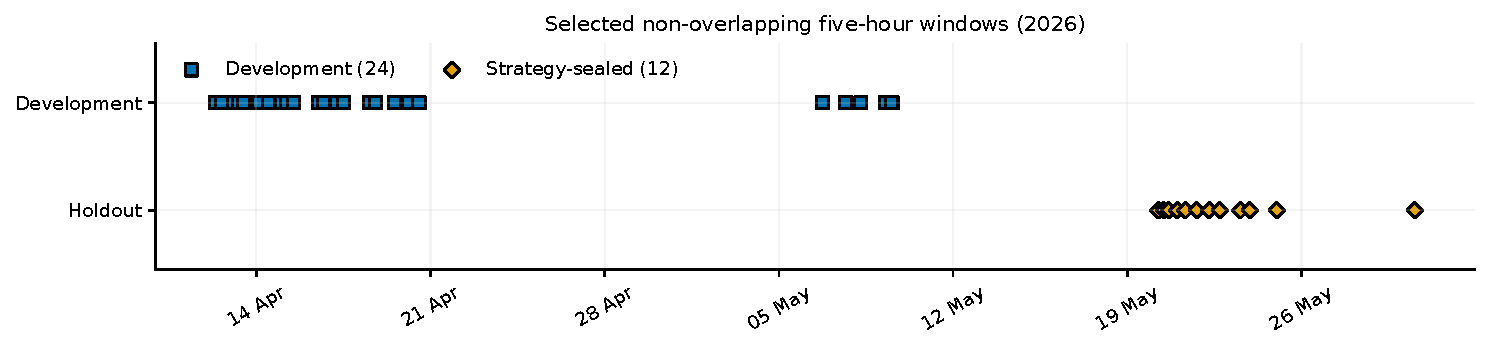
\includegraphics[width=0.96\textwidth]{figures/panel_timeline.pdf}
  \caption{Frozen selected panel. The holdout is strategy-sealed, not unseen:
  window identities and pre-strategy descriptors were examined, but no
  candidate strategy was evaluated on them. The regime comparison
  labels the holdout \emph{regime-shifted}, principally because realized
  volatility and jump counts were lower.}
  \label{fig:panel-timeline}
\end{figure}

The full integrity identity begins \texttt{\ManifestHashShort}; the selected
panel identity begins \texttt{\PanelHashShort}. Exact SHA-256 values and every
selected start are committed in the canonical artifacts.

A publication-time audit hash-checked all 120 selected development depth files.
Every snapshot bridged. The first later local depth receipt followed the legacy
tag by a median \SnapshotReceiptMedianMs{} ms, 90th percentile
\SnapshotReceiptPninetyMs{} ms, and maximum \SnapshotReceiptMaxMs{} ms. This is
an upper-bound response-completion proxy, not a measured round trip. Frozen
fills associated with orders placed before the selected policy boundary numbered
\SnapshotPreBridgeFillsQcZero{} at $c=0$ and
\SnapshotPreBridgeFillsQcOne{} at $c=1$. This is a proxy diagnostic, not an upper
bound or a robustness result, and it cannot exclude changed queue age. In all
120 files the selected policy boundary was the valid bridge, but its replay time
remains exchange \code{E}. The full V3 panel must be rerun under the new policy.

\subsection{Data availability}

Raw recordings are not stored in Git. At the report date the complete local
multi-dataset capture is approximately 37 GB, including unused
perpetual-futures data. The two spot directories used here occupy approximately
20.5 GB; the 240 selected development files occupy approximately 0.82 GB. The
tracked repository contains only selected derived artifacts. This gives three
distinct reproducibility levels:

\begin{enumerate}
  \item a fresh clone can run deterministic unit tests and a synthetic
        event-driven lifecycle demo;
  \item a fresh clone can validate the committed artifact structure, expected
        identities and verdict fields, regenerate report figures, and confirm
        that no candidate holdout artifact exists; and
  \item reproducing replay-derived numbers requires the locally held raw files
        whose hashes are recorded in the integrity manifest.
\end{enumerate}

The repository therefore uses the precise term \emph{artifact-verifiable}; it
does not claim that the full empirical panel can be rerun from a clone alone.

\subsection{End-to-end architecture}

Figure \ref{fig:architecture} shows the main information flow. Strategies
express intent through order or cancellation requests. The execution simulator,
not the strategy, owns arrival time, order state, queue position, fills, and
fees. This boundary keeps trading logic independent of execution mechanics and
makes it possible to test the latter with synthetic event paths.

\begin{figure}[H]
\centering
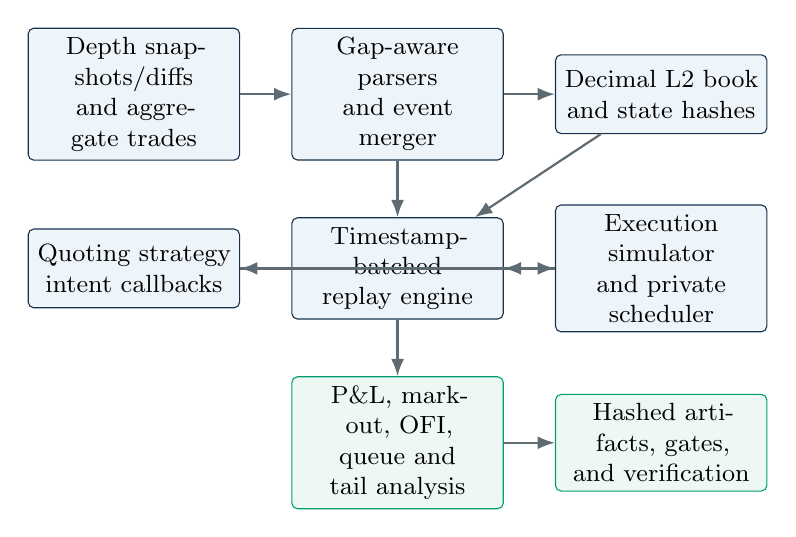
\begin{tikzpicture}[
  node distance=0.72cm and 0.65cm,
  box/.style={draw=Navy, rounded corners=2pt, fill=PaleBlue, align=center,
              minimum height=1.0cm, text width=2.45cm, font=\small},
  analysis/.style={draw=BluishGreen, rounded corners=2pt, fill=PaleTeal, align=center,
                   minimum height=1.0cm, text width=2.45cm, font=\small},
  arrow/.style={-{Latex[length=2.2mm]}, thick, draw=Slate}
]
  \node[box] (raw) {Depth snapshots/diffs\\and aggregate trades};
  \node[box, right=of raw] (parse) {Gap-aware parsers\\and event merger};
  \node[box, right=of parse] (book) {Decimal L2 book\\and state hashes};
  \node[box, below=of parse] (engine) {Timestamp-batched\\replay engine};
  \node[box, left=of engine] (strategy) {Quoting strategy\\intent callbacks};
  \node[box, right=of engine] (sim) {Execution simulator\\and private scheduler};
  \node[analysis, below=of engine] (analysis) {P\&L, markout, OFI,\\queue and tail analysis};
  \node[analysis, right=of analysis] (artifacts) {Hashed artifacts, gates,\\and verification};

  \draw[arrow] (raw) -- (parse);
  \draw[arrow] (parse) -- (book);
  \draw[arrow] (parse) -- (engine);
  \draw[arrow] (book) -- (engine);
  \draw[arrow] (engine) -- (strategy);
  \draw[arrow] (strategy) -- (sim);
  \draw[arrow] (sim) -- (engine);
  \draw[arrow] (engine) -- (analysis);
  \draw[arrow] (analysis) -- (artifacts);
\end{tikzpicture}
\caption{System architecture. Recorded market data and simulated private
actions meet on the deterministic modeled clock defined in Section~4.}
\label{fig:architecture}
\end{figure}

\subsection{Component responsibilities}

\begin{table}[H]
\centering
\caption{Primary code boundaries.}
\begin{tabularx}{\textwidth}{@{}L{0.29\textwidth}Y@{}}
\toprule
Component & Responsibility \\
\midrule
\artifact{src/replay/orderbook.py} & Sorted aggregate depth, best prices and sizes, mid, spread, microprice, snapshots/diffs, deterministic state hash. \\
\artifact{src/replay/depth_parser.py} & Hourly depth decoding, snapshot bridging, stale-diff rejection, and sequence-gap propagation across files. \\
\artifact{src/replay/trade_parser.py} & Aggregate-trade decoding, modeled ordering field, aggressor side, and ID-gap detection. \\
\artifact{src/replay/event_merger.py} & Stable two-way market-data merge and the recorded depth-before-trade tie rule. \\
\artifact{src/replay/engine.py} & Timestamp grouping, book mutation, strategy callbacks, private-action scheduling, gap policy, and replay termination. \\
\artifact{src/execution/simulator.py} & Entry/cancel latency, order lifecycle, post-only checks, FIFO queue state, partial fills, volume conservation, and fees. \\
\artifact{src/strategies/base_mm.py} & Inventory and live-order tracking, tick rounding, requote behavior, and the hard working-exposure envelope. \\
\directory{src/analysis} & Markouts, P\&L decomposition, matched lots, bootstrap intervals, OFI/microprice tests, fee and queue sensitivity, and tail diagnostics. \\
\bottomrule
\end{tabularx}
\end{table}

\subsection{Determinism}

Prices, quantities, fees, queue ranks, and accounting use
\code{decimal.Decimal}. Latency jitter uses seeded independent random streams
for entries and cancels. Replay uses recorded timestamps without runtime clock
reads. Every
checkpoint hashes a canonical serialization of full book state. Determinism is
necessary for debugging, regression testing, artifact identity, and eventual
cross-language parity; it does not by itself validate the economic assumptions
of the simulator.

\section{Execution-Model Contract}

\subsection{Why execution is part of the estimand}

For a passive maker, the fill set is generated jointly by market events and the
simulator's rules. Changing arrival timing, cancellation timing, queue
advancement, or post-only handling can change which trades fill an order. It can
therefore change P\&L, markouts, conditional signal tests, and apparent latency
sensitivity. Execution assumptions are not an implementation footnote; they
define the sample on which the strategy is evaluated.

L2 data reports aggregate quantity at a price, not individual order identities.
No replay using this dataset observes true queue rank. The implementation is a
documented execution approximation, not an exchange twin.

\subsection{Historical and current semantics}

\begin{table}[H]
\centering
\caption{Execution-model boundary.}
\label{tab:model-comparison}
\begin{tabularx}{\textwidth}{@{}L{0.25\textwidth}YY@{}}
\toprule
Feature & \LegacyModel & \CurrentModel \\
\midrule
New-order arrival & Eligible on the next depth update after modeled arrival & Scheduled at the exact arrival millisecond on the model clock \\
Cancellation & Effective immediately when requested & Scheduled separately; order stays fillable while cancel is in flight \\
Cancel/fill race & Absent & Explicit; a fill can beat a late cancel \\
Equal-time private action & Implicit through depth activation & All recorded market data at the millisecond precedes private arrivals \\
Own orders at one price & Incomplete separation of public and own queue & Non-overlapping own FIFO ranks with trade-volume conservation \\
Gap state & Strict replay policy added, but legacy artifacts retain old private semantics & Whole timestamp group invalidated fail-closed until snapshot resync \\
Snapshot timing & Returned state applied at a pre-fetch local tag & Local request-time resync barrier; recovery gated by post-response receipt order and released on depth \code{E}; new captures store request and response times \\
Artifact root & \path{results/panels/btcusdt_l2_panel_v2} & \path{results/panels/btcusdt_l2_panel_v3_event_driven} \\
Research status & Frozen historical evidence & Mechanics accepted; economic rerun pending \\
\bottomrule
\end{tabularx}
\end{table}

\subsection{Clock and equal-timestamp policy}

The replay clock has two classes of event. Its recorded-data axis combines local
request time for fail-closed resync barriers, depth \code{E} for ordinary diffs
and recovered-state release, and trade \code{T} for trades:

\begin{enumerate}
  \item recorded market data, ordered depth before trade for unresolved
        millisecond ties and preserving source order within each stream; and
  \item simulated private arrivals for new orders and cancellations, preserving
        stable insertion order.
\end{enumerate}

Private actions strictly before a market-data timestamp are processed first.
At an identical millisecond, the complete recorded market-data group is
processed before private arrivals. A new order arriving at the same millisecond
as a trade is therefore not eligible for that trade; a cancel arriving at the
same millisecond loses the race. This is a conservative policy for unresolved
timestamps, not a statement about the venue's internal matching sequence.

\begin{figure}[H]
\centering
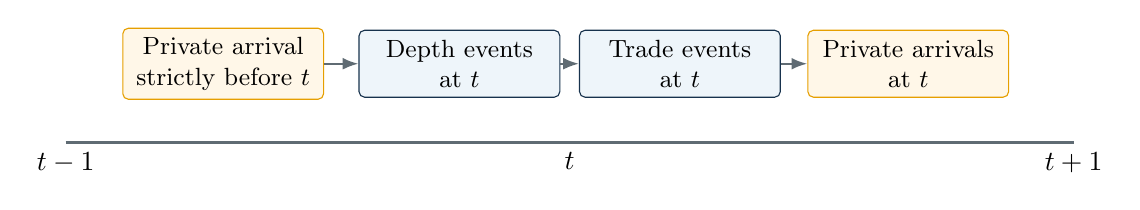
\begin{tikzpicture}[
  event/.style={draw=Navy,rounded corners=2pt,fill=PaleBlue,align=center,
                minimum width=2.55cm,minimum height=0.85cm,font=\small},
  private/.style={draw=Orange,rounded corners=2pt,fill=PaleOrange,align=center,
                  minimum width=2.55cm,minimum height=0.85cm,font=\small},
  arrow/.style={-{Latex[length=2mm]},thick,draw=Slate}
]
  \draw[thick,Slate] (0,0) -- (12.8,0);
  \node[below] at (0,0) {$t-1$};
  \node[below] at (6.4,0) {$t$};
  \node[below] at (12.8,0) {$t+1$};
  \node[private] (before) at (2.0,1.0) {Private arrival\\strictly before $t$};
  \node[event] (depth) at (5.0,1.0) {Depth events\\at $t$};
  \node[event] (trade) at (7.8,1.0) {Trade events\\at $t$};
  \node[private] (equal) at (10.7,1.0) {Private arrivals\\at $t$};
  \draw[arrow] (before) -- (depth);
  \draw[arrow] (depth) -- (trade);
  \draw[arrow] (trade) -- (equal);
\end{tikzpicture}
\caption{\CurrentModel\ timestamp policy. The horizontal placement inside
the $t$ group shows processing precedence, not sub-millisecond observation.}
\label{fig:timestamp-policy}
\end{figure}

Depth-decrease attribution is deferred until every trade at the same
millisecond has been observed. Otherwise the depth-before-trade rule could
mistake traded quantity for a cancellation and grant queue improvement twice.

\subsection{Order and cancellation lifecycle}

Submitting an \code{OrderRequest} creates a pending order and schedules its
arrival at
\begin{equation}
  t_{\mathrm{arrive}} = t_{\mathrm{submit}} + L_e + J_e,
\end{equation}
where $L_e$ is base entry latency and $J_e$ is a seeded uniform integer jitter
bounded so that delay cannot be negative. Cancellation uses a separate latency
and independent random stream:
\begin{equation}
  t_{\mathrm{cancel}} = \max\left(t_{\mathrm{request}} + L_c + J_c,
  t_{\mathrm{arrive}}\right).
\end{equation}

While entry is pending, its quantity is counted as potential exposure but it is
not eligible for market fills. Once active, the order remains fillable until
the cancellation reaches the simulated exchange. Lifecycle events distinguish
request from effect:
\code{cancel_requested}, \code{cancelled}, and \code{cancel_too_late}. A
post-only limit that would cross on arrival is cancelled with an explicit
reason rather than silently reclassified as a passive fill.

\subsection{Queue model and own-order FIFO}

When a resting order arrives, its modeled quantity ahead is decomposed as
\begin{equation}
  Q^{\mathrm{ahead}}_i = Q^{\mathrm{external}}_i + Q^{\mathrm{own}}_i.
\end{equation}
The external component starts from displayed L2 quantity, subject to a FIFO
floor imposed by earlier live own orders. The own component is the remaining
quantity of earlier simulated orders at the same side and price. A public depth
decrease not explained by recorded trades improves only the external component:
\begin{equation}
  Q^{\mathrm{external}}_{i,t+1}
  = Q^{\mathrm{external}}_{i,t}\left(1-c\rho_t\right),
  \qquad c\in[0,1],
\end{equation}
where $c$ is queue-cancellation credit and $\rho_t$ is the inferred fraction of
the displayed queue removed without matching trade volume. The two historical
endpoints are $c=0$ and $c=1$; neither is claimed to be calibrated ground truth.

Recorded trade quantity advances non-overlapping FIFO ranks. The simulator
plans and validates the complete transition before mutating any order and
asserts
\begin{equation}
  \sum_i q^{\mathrm{maker\ fill}}_{i,t}
  \le q^{\mathrm{recorded\ trade}}_t.
\end{equation}
Cancelling an earlier own order releases its unfilled quantity from later own
queues. Decimal comparisons use only a scale-aware $10^{-24}$ relative
tolerance for division residue; the tolerance cannot create fill budget.

\subsection{Risk envelope}

Position is not the only relevant exposure during cancel/replace. If multiple
same-side entries are pending or cancels are in flight, all may still fill. The
strategy therefore checks worst-case working exposure:
\begin{equation}
  \left|I_t + \sum_{i\in\mathcal{F}_t^{\mathrm{same}}}
  s_i q^{\mathrm{remaining}}_i + s_{\mathrm{new}}q_{\mathrm{new}}\right|
  \le I_{\max},
\end{equation}
where $\mathcal{F}_t^{\mathrm{same}}$ includes active orders, pending entries
that may become fillable, and active orders with cancels in flight. An invariant
breach aborts replay; it is not recorded as a harmless temporary overshoot.

\subsection{Gaps and replay termination}

A known sequence gap invalidates the entire timestamp group before any event in
that group can fill an order or invoke strategy logic. Local orders and pending
actions become invalid because their queue state is no longer trustworthy.
Replay resumes only at a valid snapshot. This is fail-closed research
bookkeeping, not a claim that the exchange cancelled those orders instantly.

Private events scheduled after the last recorded market event are not executed
against an assumed future book. Remaining live orders are terminalized as
expired, and pending action counts are reported separately.

\subsection{Known execution limits}

\begin{itemize}
  \item Aggregate L2 cannot reveal true market-by-order rank, hidden liquidity,
        or where cancellations occurred relative to the simulated order.
  \item The modeled clock mixes recorded local request time for resync barriers,
        depth event time \code{E} for release and ordinary diffs, trade matching
        time \code{T}, and local receipt order used to gate snapshots.
        Those fields are not guaranteed to be perfectly comparable, and
        millisecond resolution cannot identify true within-millisecond matching
        order. The post-response receipt gate removes request-start placement,
        but its selected boundary remains on exchange \code{E}; it does not
        calibrate client observation or feed latency.
  \item Market-data latency is not modeled separately from private-message
        latency.
  \item Counterfactual taker execution shares a shadow liquidity ledger only
        until the next observed depth update; taker-heavy research needs market
        impact and stronger book reconciliation.
  \item No execution model here has been calibrated against live order
        acknowledgements and fills from an exchange account.
\end{itemize}

\section{Research Design}

\subsection{Primary quantities}

Let best bid and ask be $b_t$ and $a_t$, with displayed top-level quantities
$q^b_t$ and $q^a_t$. The arithmetic mid and microprice are
\begin{equation}
  m_t=\frac{b_t+a_t}{2}, \qquad
  \mu_t=\frac{q^b_ta_t+q^a_tb_t}{q^b_t+q^a_t}.
\end{equation}
Microprice deviation is $(\mu_t-m_t)/m_t\times10^4$ bps. For horizon $h$,
the population response is forward mid drift,
\begin{equation}
  r_{t,h}=10^4\frac{m_{t+h}-m_t}{m_t}.
\end{equation}

The top-of-book OFI increment follows the event construction in
\citet{cont2014}:
\begin{align}
 e_n={}&\mathbf{1}_{b_n\ge b_{n-1}}q^b_n
       -\mathbf{1}_{b_n\le b_{n-1}}q^b_{n-1} \\
     &-\mathbf{1}_{a_n\le a_{n-1}}q^a_n
       +\mathbf{1}_{a_n\ge a_{n-1}}q^a_{n-1}.
\end{align}
Raw one-second OFI sums $e_n$ over the preceding second. Normalized OFI divides
that sum by mean displayed best-bid-plus-best-ask depth over the contributing
updates. The code definition is in \artifact{src/analysis/ofi_signal.py}.

For a maker fill $i$, let $s_i=+1$ for a buy and $-1$ for a sell. The
fill-conditioned response is
\begin{equation}
  z_{i,h}=10^4s_i\frac{m_{i+h}-m_{i^-}}{m_{i^-}},
\end{equation}
where $m_{i^-}$ is the latest book sample strictly before the fill. This
quantity isolates subsequent mid movement from transaction-price spread
capture. The separate standalone markout diagnostic uses fill price as its
reference and is not substituted into this premise test.

Strictly-pre-fill anchoring is enforced in both the OFI window and reference
mid. A book sample stamped at the fill millisecond is excluded, because it can
already contain the same-millisecond market move associated with the simulated
fill. Tests contain a leakage tripwire for this boundary.

\subsection{Baseline and development panel}

The frozen baseline is a post-only \code{MicropriceMM} on Binance spot
BTCUSDT. It quotes 0.001 BTC on each eligible side, 2 USDT from microprice,
requotes at most every five seconds, and caps position at 0.01 BTC. Historical
execution assumptions are 10 ms entry latency without jitter, a 2 bps maker
fee, a 5 bps taker fee, and queue-cancellation credit evaluated at $c=0$ and
$c=1$. Each nominal five-hour window is the sum of five independently initialized
one-hour replay episodes. Strategy, execution, and inventory state restart each
hour; residual inventory is marked to the session-end mid and then discarded
without a modeled liquidation. The five-hour value is therefore an inference
cluster, not continuous five-hour portfolio P\&L. Latency and fees are modeled
inputs, not measurements from the author's exchange account.

The 2 USDT / five-second baseline was selected during an exploratory April
anchor analysis. Six such anchors were retained among the 24 development
windows. The expanded panel therefore reduces dependence on those examples but
is not an untouched confirmation sample. That qualification is important when
interpreting the later confidence intervals.

\begin{figure}[H]
  \centering
  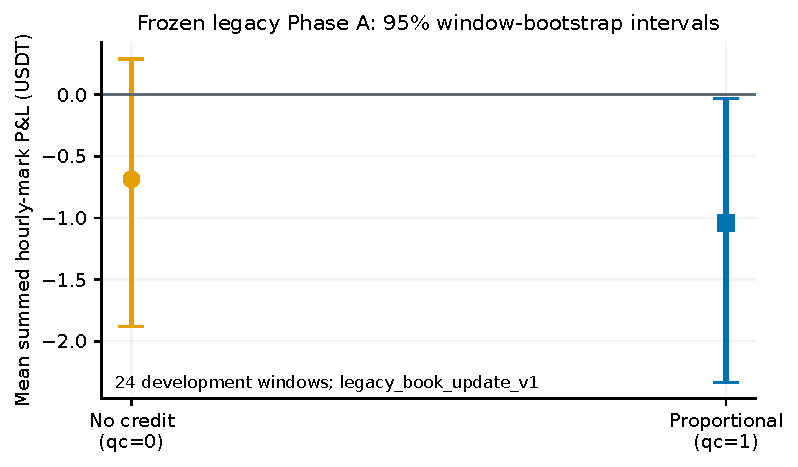
\includegraphics[width=0.78\textwidth]{figures/phase_a_ci.pdf}
  \caption{Phase A estimand: the mean full-strategy net P\&L across 24
  five-hour development windows. Intervals resample windows, not individual
  events.}
  \label{fig:phase-a-ci}
\end{figure}

\subsection{Sequential decision protocol}

The Phase A/B/C sequence and thresholds were written into the repository
before their associated evaluation. This is a pre-specified protocol in the
repository history; it is not an externally registered study.

\begin{enumerate}
  \item \textbf{Phase A---baseline remeasurement.} Estimate mean net P\&L and a
        95\% nonparametric interval by resampling the 24 five-hour windows
        10,000 times with seed 7, separately at $c=0$ and $c=1$.
  \item \textbf{Phase B---premise first.} Before running a strategy that acts
        on OFI, require a stable population association and a material
        fill-conditioned separation. If the premise fails, do not search the
        candidate's thresholds.
  \item \textbf{Phase C---model stress.} Sweep queue-cancellation credit at
        $\{0,.25,.5,.75,1\}$ under 10 ms latency, plus $\{0,50\}$ ms at the two
        credit endpoints. Compare throughput, matched-lot economics, and
        full-strategy P\&L.
\end{enumerate}

The primary one-second normalized-OFI population gate required all of:

\begin{itemize}
  \item one coefficient sign in at least 75\% of development windows;
  \item pooled HAC $|t|\ge2$; and
  \item at least 0.05 bps predicted drift for one signal standard deviation.
\end{itemize}

The conditional gate compared, at 30 seconds, the most-populated negative
side-aligned bucket with the most-populated nonnegative bucket. It required
the latter's mean $z_{i,30s}$ to exceed the former by at least 1.0 bps, with at
least 30 observations in each selected bucket. The 1.0 bps threshold is a
research materiality heuristic and 30 is a minimum-count rule; neither is a
formal power calculation. The chosen comparison also does not test the two
extreme buckets. For those reasons the complete bucket response, its
monotonicity, and its counts must accompany the mechanical gate result.

\subsection{Dependence and uncertainty}

Overlapping forward returns are serially dependent. Pooled regressions
therefore report Newey--West heteroskedasticity-and-autocorrelation-consistent
standard errors \citep{neweywest1987}. The implementation takes the larger of
the overlap-horizon lag count and the Newey--West sample-size rule, capped only
at $n-1$. This corrects standard errors for the specified local dependence
structure, but it does not turn millions of one-second observations into
millions of independent market regimes. The pooled population regression does
not yet carry window-clustered uncertainty across market regimes.

Phase A uncertainty instead resamples whole five-hour windows, preserving
within-window dependence \citep{efron1979}. With only 24 clustered windows,
the interval describes variation within this mechanically selected panel; it
does not estimate sampling variation from a random population of market
regimes. A
future inference pass should add window-clustered uncertainty to both the pooled
population effect and the fill-conditioned bucket contrast rather than
interpreting their raw event counts as independent precision.

\subsection{Holdout discipline}

Twelve late-May windows were selected and their identities hashed alongside
the development panel. This holdout is strategy-sealed rather than unseen. A
pre-strategy regime screen labeled it
\code{regime-shifted}; it had lower realized volatility and fewer jumps than
development. The holdout protocol requires a candidate, parameters, gate
result, and commit to be locked before one evaluation. Because the OFI premise
gate blocked the only candidate, the template remains unlocked and no holdout
strategy output exists. No candidate evaluation was run---there is no favorable
or unfavorable strategy result kept off the page.

\section{Frozen Development Results}

\begin{cautionbox}
\textbf{Provenance.} Every number in this section belongs to the frozen V2
artifact root and historical execution model. These are results of that
experiment, not estimates from the current simulator. V2 also applied REST
snapshot state at a pre-fetch local tag. The timing proxy audit does not prove
that its execution-derived values are invariant to the post-response-gated
exchange-clock policy.
\end{cautionbox}

\subsection{Phase A: passive baseline}

The fixed microprice maker was unprofitable in 18 of 24 windows at both queue
endpoints. Table \ref{tab:phase-a} reports window means and 95\% bootstrap
intervals. Proportional cancellation credit produced a wholly negative
interval. The no-credit interval crossed zero, but its point estimate was also
negative. No stable passive edge was demonstrated. This conclusion retains the
queue-model dependence of the uncertainty.

The fee hurdle is economically central. At a representative 71,500 USDT price,
the 2 USDT half-spread is about 0.28 bps per side, while the simulation charges
2 bps per maker fill. In the pooled fee diagnostic, completed matched lots would
break even at maker fees of \MatchedBreakEvenQcZero\ bps under no cancellation
credit and \MatchedBreakEvenQcOne\ bps under proportional credit. Including the
hourly residual-inventory marks, the full strategy would instead require maker
rebates of \FullRebateQcZero\ and \FullRebateQcOne\ bps,
respectively. The baseline is therefore a demanding execution diagnostic, not a
configuration with an assumed spread advantage over fees.

The frozen fee summary metadata calls this a ``window-close'' mark. That phrase
is a preserved wording error: the computation marks each one-hour session end
and resets state before the next session. The numeric rows are unchanged.

\begin{table}[H]
\centering
\caption{Frozen legacy Phase A full-strategy net P\&L per nominal five-hour
development window. Each row sums five independently initialized, hourly marked
episodes (0.001 BTC quotes, 0.01 BTC maximum position, 2 bps maker fee).}
\label{tab:phase-a}
\begin{tabular}{@{}lrrr@{}}
\toprule
Queue credit & Mean (USDT) & 95\% CI low & 95\% CI high \\
\midrule
0 (no credit) & \PhaseAQcZeroMean & \PhaseAQcZeroLow & \PhaseAQcZeroHigh \\
1 (proportional) & \PhaseAQcOneMean & \PhaseAQcOneLow & \PhaseAQcOneHigh \\
\bottomrule
\end{tabular}
\end{table}

The original reference was microprice because it can encode top-of-book
imbalance. Its own one-second signal was nevertheless weak: $+0.0190$ bps per
signal standard deviation, HAC $t=1.74$, with a positive coefficient in 19 of
24 windows. It missed both the $|t|\ge2$ and 0.05 bps materiality gates. This
motivated OFI as a richer event-flow signal without claiming that the baseline
was optimized out of trouble.

\subsection{Phase B: OFI population evidence}

Normalized OFI passed all three population gates. The one-second coefficient
was positive in 24 of 24 windows. Its unconditional bucket response rose
monotonically from $-0.276$ bps in the lowest bucket to $+0.284$ bps in the
highest. Table \ref{tab:ofi-regression} shows that statistical significance
persists at longer horizons while explanatory power falls sharply.

\begin{table}[H]
\centering
\caption{Frozen legacy pooled normalized-OFI regressions on forward mid drift.}
\label{tab:ofi-regression}
\begin{tabular}{@{}lrrrr@{}}
\toprule
Horizon & Observations & Slope & HAC $t$ & Effect / 1 s.d. (bps) \\
\midrule
1 s  & 430,278 & 0.1192 & 64.63 & 0.1233 \\
10 s & 430,062 & 0.2424 & 35.83 & 0.2507 \\
1 m  & 428,862 & 0.3157 & 18.06 & 0.3268 \\
5 m  & 423,102 & 0.2958 &  7.48 & 0.3069 \\
\bottomrule
\end{tabular}
\end{table}

The one-second regression $R^2$ is only \OFIRSquared. The large $t$-statistic
reflects a repeatable short-horizon association in a densely sampled series. It
does not imply that the signal explains most price variation or can be captured
after execution and costs.

\begin{figure}[H]
  \centering
  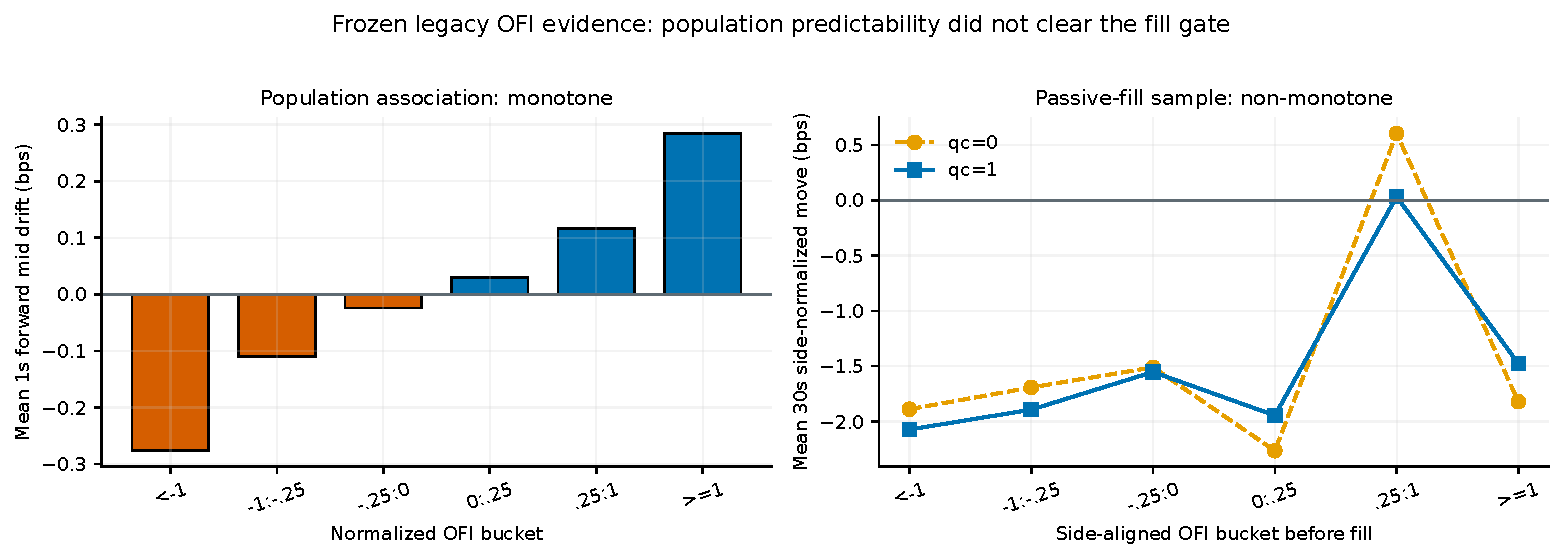
\includegraphics[width=0.98\textwidth]{figures/ofi_population_vs_fills.pdf}
  \caption{Unconditional and fill-conditioned OFI evidence. The left panel is
  queue-independent. The right panel uses historical baseline fills and must
  be interpreted under the legacy execution model.}
  \label{fig:ofi-population-fill}
\end{figure}

\subsection{Phase B: the conditional gate}

The pre-specified 30-second conditional comparison was only
\OFIConditionalQcOne\ bps at $c=1$ and \OFIConditionalQcZero\ bps at $c=0$,
far below 1.0 bps. Its selected bucket counts were respectively
\OFIMinCountQcOne\ and \OFIMinCountQcZero, exceeding the minimum-count rule.
The full response was not monotone. In particular, the smaller
$[0.25,1)$ bucket appeared more favorable than the selected adverse bucket at
both endpoints, but had only 71 and 54 observations. That is an exploratory
pattern, not a post-hoc replacement for the defined test and not a powered
estimate of a tradeable threshold.

The defensible result is consequently precise: the defined fill-conditioned
gate failed at both queue endpoints, and the broader bucket pattern was not
stable or monotone enough to advance the candidate. It would be too strong to
say that OFI's predictive content universally ``vanished'' on fills, or that an
unrun \code{OFIGatedMM} necessarily loses.

\subsection{Phase C: queue and latency stress}

At 10 ms entry latency, granting more cancellation credit raised modeled fill
throughput but worsened both quantity-weighted matched-lot economics and total
strategy P\&L. This monotone economic deterioration is stronger evidence than
the sign flip observed in the earlier six-anchor analysis.

\begin{table}[H]
\centering
\caption{Frozen legacy pooled Phase C results at 10 ms. ``Orders/fill'' is a throughput
diagnostic, matched net/BTC weights pooled matched quantity.}
\label{tab:queue-stress}
\begin{tabular}{@{}rrrrr@{}}
\toprule
Credit & Fills & Orders/fill & Matched net/BTC & Full net P\&L \\
\midrule
0.00 & 1,595 & 70.8 &  $-9.75$ & $-16.46$ \\
0.25 & 1,796 & 62.9 & $-15.08$ & $-17.64$ \\
0.50 & 1,802 & 62.6 & $-16.08$ & $-20.88$ \\
0.75 & 1,831 & 61.6 & $-17.51$ & $-21.33$ \\
1.00 & 2,041 & 55.4 & $-23.65$ & $-25.03$ \\
\bottomrule
\end{tabular}
\end{table}

\begin{figure}[H]
  \centering
  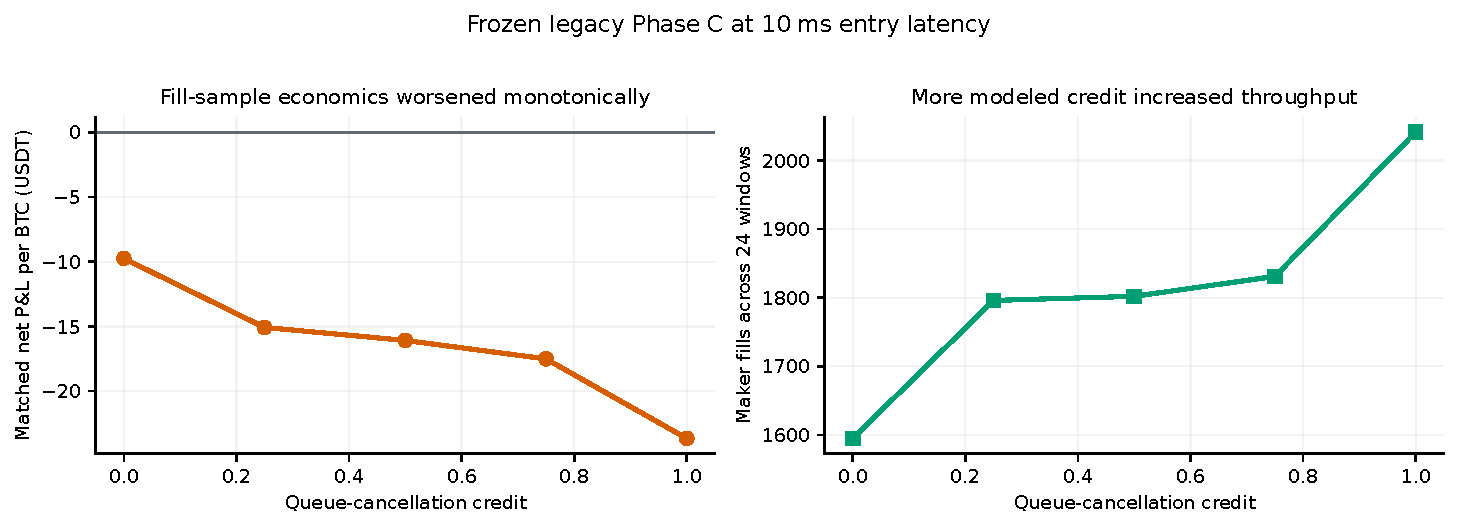
\includegraphics[width=0.92\textwidth]{figures/queue_credit_stress.pdf}
  \caption{Queue-credit sensitivity. More favorable modeled queue advancement
  selects a larger pooled fill sample with worse mean matched economics. The
  sweep does not establish that fill sets are nested.}
  \label{fig:queue-stress}
\end{figure}

The historical $0/10/50$ ms entry-latency sweep was numerically unchanged at
the two credit endpoints. Under \LegacyModel, order eligibility was quantized
to the next depth update, so this is evidence about a model limitation rather
than evidence that real latency is irrelevant. It was one reason to build the
event-driven clock.

\subsection{Tails and bounded replay audits}

Under proportional credit, the worst 5\% of 30-second fill observations
accounted for 40.64\% of the summed adverse movement. The worst 5\% of matched
lots accounted for 86.62\% of total matched-lot loss. Fill toxicity was thus
broad with meaningful tails, whereas realized matched-lot loss was far more
tail-concentrated. These ratios depend on the signed-total denominator and are
reported with negative-only denominators in the artifacts as well.

The panel-wide same-millisecond audit found 10 overlap fills among 2,041 fills
at $c=1$ (0.49\%) and 7 among 1,595 at $c=0$ (0.44\%). It found zero
\emph{artifact-evidenced} contradictions of the depth-before-trade assumption.
That bounded label matters: reconciliation artifacts do not persist every
queue-drain timestamp, so candidate rows cannot all be adjudicated after the
fact. Separately, all six original anchor windows were aggregate-trade-gap
clean, and replaying them under the later fail-closed trade-gap policy changed
no reported value.

\subsection{Decision}

No strategy advanced. The baseline did not demonstrate stable positive
economics, microprice was weak, and OFI cleared the population screen but not
the specified execution-conditioned premise. Phase C showed that reasonable
variation in unobserved queue advancement changed throughput and loss magnitude
without producing positive pooled matched economics. No candidate strategy was
evaluated on the holdout. This is a negative/conditional development result,
not a live-performance claim.

\section{Failure Analysis and Lessons}

\subsection{What changed after apparent success}

The project is most informative when read as a sequence of claims that became
more constrained as the measurement system improved.

\begin{table}[H]
\centering
\caption{Material failure modes and their disposition.}
\begin{tabularx}{\textwidth}{@{}L{0.22\textwidth}YY@{}}
\toprule
Issue & Why it mattered & Resolution \\
\midrule
Accidental taker fills & Entry latency could make intended passive limits cross, creating attractive but irrelevant execution. & Post-only is the default; crossing arrivals terminate with an explicit reason. \\
Naive snapshot synchronization & Stale post-snapshot diffs could roll the reconstructed book backward. & Stale diffs are dropped, the first retained diff must bridge, and parser tests cover both rules. \\
Pre-fetch snapshot tags & The recorder stamped request start, then blocked on REST; legacy replay could apply returned state before response completion. & Frozen V2 is labeled; current recovery is gated by post-response receipt order, future captures store both timestamps, and a 120-hour proxy audit is committed. \\
Trade-ID gaps & Missing aggressor trades can overstate queue position and suppress fills. & New research pauses fail-closed, invalidates local state, and resumes only at a valid snapshot; six anchors were audited before/after. \\
Same-ms fill leakage & A fill-time book sample could include the causal trade and leak its move into prior OFI. & Conditional OFI and its reference mid are strictly before the fill; a test guards the boundary. \\
Private-event quantization & Legacy entry arrival waited for a depth event and cancels had no delay, masking races and latency sensitivity. & Historical results were frozen and labeled; \CurrentModel\ added explicit millisecond scheduling and a new artifact namespace. \\
Own-order overlap & Multiple simulated orders could compete for the same recorded trade or obscure working exposure. & Current replay separates public and own queue, conserves trade volume, models own FIFO, and checks all fillable same-side quantity. \\
Publication overstatement & Phase 1 ratios and the OFI headline could imply stronger evidence than the implementation supports. & Phase 1 is now an educational precursor; the OFI conclusion is stated as a failed defined gate with non-monotone conditional evidence. \\
\bottomrule
\end{tabularx}
\end{table}

When a correction could change the estimand, the project did not silently
overwrite the interpretation. Contaminated outputs were superseded, corrected
studies were regenerated, and the private-timing change created an explicit
model version. That separation is essential for an auditable research record.

\subsection{Empirical limitations}

\begin{itemize}
  \item \textbf{One venue and instrument.} Evidence comes from Binance spot
        BTCUSDT and cannot establish cross-venue or cross-asset robustness.
  \item \textbf{Short, clustered period.} Development windows lie mainly in
        two April/May clusters; calendar, volatility, and market-structure
        coverage is limited.
  \item \textbf{Selective availability.} Only 775 of 1,193 inventoried hours
        passed the data requirements. Missingness may correlate with volatile
        or operationally difficult periods.
  \item \textbf{Exploration inside development.} Six baseline-selection
        anchors remain in the 24-window panel; results are not a pristine
        confirmatory replication.
  \item \textbf{Hourly state resets.} Each five-hour value sums five independent
        one-hour episodes. Residual inventory is marked at each session end and
        discarded without liquidation cost, so the result is not continuous
        five-hour portfolio P\&L.
  \item \textbf{Strategy-sealed but shifted holdout.} The 12 late-May windows are lower
        volatility and have not been used for a candidate.
  \item \textbf{Limited conditional inference.} The OFI bucket minimum is not
        a power analysis, the defined contrast is not an extreme-to-extreme
        comparison, and a window-clustered interval for that contrast remains
        future work.
  \item \textbf{Pooled-signal inference.} Newey--West errors address specified
        local serial dependence, not uncertainty across independently sampled
        market regimes; a window-clustered population-effect interval remains
        future work.
\end{itemize}

\subsection{Model limitations}

Aggregate L2 supplies displayed quantity, not order identities. The true queue
rank of a hypothetical order is unobservable, and cancellation credit brackets
one uncertainty without calibrating it. Hidden liquidity, iceberg refresh,
self-trade prevention, exchange throttles, acknowledgement latency, network
jitter, message loss, and venue-specific matching details are absent. The
millisecond tie rule is deterministic but cannot recover sub-millisecond truth.

The simulator assumes the recorded public market remains unchanged by the
strategy. That is reasonable only for very small passive orders. It is not a
market-impact model, a capacity study, or a production matching-engine replica.
The 2 bps maker fee is a fixed assumption rather than an observed account-tier
fee. It is also large relative to the 2 USDT half-spread at the observed BTC
price level, making fee calibration load-bearing.

\subsection{Software and operational limits}

The current Python implementation is a tested behavioral reference. It favors
explicit state and \code{Decimal} arithmetic over throughput, has not been
profiled as a low-latency system, and is not connected to an order gateway.
Tests cover deterministic synthetic paths and artifact contracts; they do not
replace exchange conformance tests, live shadowing, chaos testing, a production
gateway, kill switch, monitoring, or other operational risk controls.

Raw data is not distributable from this repository, so a fresh clone can verify
committed evidence but cannot independently reconstruct every economic number.
The data statement records this boundary and the expected local layout.

\subsection{Technical lessons}

Five lessons carry forward:

\begin{enumerate}
  \item execution determines the sample, so a predictor must be tested on the
        fills it can actually influence;
  \item a simulator assumption should be versioned whenever it can change order
        eligibility or queue state;
  \item negative results become useful when their stop rule and provenance are
        inspectable;
  \item sensitivity analysis should report selection effects---throughput and
        fill composition---not just a final P\&L number; and
  \item performance work should begin only after a deterministic behavioral
        contract exists to serve as an oracle.
\end{enumerate}

These are the project's principal learnings. They are more durable than the
economic estimates from one narrow historical panel.

\section{Current Status and Reproduction}

\subsection{Where the project is now}

\begin{table}[H]
\centering
\caption{Publication-time status.}
\begin{tabularx}{\textwidth}{@{}L{0.23\textwidth}L{0.20\textwidth}Y@{}}
\toprule
Workstream & Status & Meaning \\
\midrule
Bar backtester & Educational precursor & Reusable framework and tests remain; historical performance claims are not treated as rigorous evidence. \\
Frozen L2 study & Complete under legacy model & Phase A/B/C artifacts, gates, panel identity, and audits are committed and verifiable. \\
Event-driven Python model & Mechanics accepted & Private scheduling, post-response-gated snapshot recovery, delayed cancels, own FIFO, conservation, gaps, and risk invariants pass deterministic tests. \\
V3 development economics & Pending & No execution-derived result from \CurrentModel\ is published yet. \\
Holdout & Strategy-sealed & Identities and regime descriptors were examined, but no candidate strategy run exists. \\
C++ performance port & Intentionally paused & It begins only after the Python V3 result is frozen and a separate modern C++ foundations phase is complete. \\
\bottomrule
\end{tabularx}
\end{table}

The immediate research milestone is the clean V3 development rerun under
\CurrentModel\ and \code{post_response_proxy_depth_boundary_v1}, including an explicit
before/after snapshot-timing comparison. It is not the C++ port and it is not a
holdout run.

\subsection{Fresh-clone verification}

The repository targets Python 3.11. At the 4 August 2026 checkpoint, a fresh
clone reports 376 deterministic tests passed and three optional raw-data smoke
checks skipped. All 379 pass when the selected captures are restored. From the
repository root:

\begin{lstlisting}[style=projectcode]
python3.11 -m venv .venv
source .venv/bin/activate
python -m pip install -r requirements.txt

env PYTHONPATH=. pytest -q
env PYTHONPATH=. python scripts/demo_event_driven_execution.py
env PYTHONPATH=. python scripts/verify_v2_artifacts.py
\end{lstlisting}

The synthetic simulator demo is deliberately tiny: a resting buy arrives, a
cancellation is requested, a recorded sell reaches the queue first, and the
delayed cancel is reported too late. It exercises execution lifecycle mechanics
without raw data; it does not exercise full replay timestamp batching, gap
recovery, empirical economics, or throughput.

The V2 verifier checks the manifest and panel identities, execution-model
marker, Phase A verdict, Phase B gate status, Phase C grid, same-millisecond
audit, panel-file hashes, and selected holdout identifiers across tracked
result paths and contents. It validates committed evidence; it does not
recompute replay results from raw messages.

\subsection{Building this report}

Report scalars and vector figures are regenerated only from an allowlist of
canonical frozen artifacts. The builder checks the execution-model marker and
input shape, including the distinction between 24 window rows and one pooled
row per queue/latency configuration.

\begin{lstlisting}[style=projectcode]
make report
make report-check
\end{lstlisting}

The first command rebuilds report inputs and the PDF. The second rebuilds and
then verifies that the generated asset manifest matches the committed copy.
Input/output SHA-256 values are in
\artifact{report/generated/asset_manifest.json}. The compiled document is
\artifact{report/l2_mm_research_report.pdf}.

\subsection{Full development rerun}

With the raw depth/trade layout described in \artifact{DATA.md}, the current
development runner defaults to the frozen development-window file and writes
only to the V3 namespace:

\begin{lstlisting}[style=projectcode]
env PYTHONPATH=. python scripts/run_l2_panel.py --phase all
\end{lstlisting}

Before relying on this command, use \code{--help} and inspect the committed
defaults. The runner verifies the development-panel file hash, refuses the
strategy-sealed holdout, and guards the frozen V2 directory. V3 artifact
verification remains impossible until this run produces its manifest.

\subsection{Suggested reviewer routes}

A reviewer can understand the project at three depths:

\begin{description}[leftmargin=6.2em,style=nextline]
  \item[Five minutes] Read the repository README, the executive summary, and
        the status table above.
  \item[Thirty minutes] Read Sections 3--7 and run the synthetic demo plus V2
        artifact verifier.
  \item[Code review] Start at \artifact{src/replay/engine.py} and
        \artifact{src/execution/simulator.py}; use
        \artifact{tests/test_execution_simulator.py} and
        \artifact{tests/test_engine.py} as executable specifications, then
        inspect \artifact{src/analysis/ofi_signal.py} for the research estimand.
\end{description}

\subsection{Roadmap to the performance boundary}

\begin{enumerate}
  \item Run the fixed baseline over all 24 development windows under
        \CurrentModel\ and the post-response-gated snapshot policy at both queue
        endpoints.
  \item Regenerate OFI conditional-on-fill evidence and queue/latency stress,
        then compare fill identity and economics with the legacy study.
  \item If a candidate clears a newly committed development rule, lock it and
        perform the one-shot holdout strategy evaluation; otherwise close the
        research arc without evaluating a candidate there.
  \item Freeze a deterministic Python reference, golden event traces, artifact
        schemas, and parity tolerances.
  \item Complete a separate modern C++ foundations phase before implementing
        any hot-path port. Later performance work must reproduce the Python
        contract before it is benchmarked.
\end{enumerate}

\enlargethispage{4\baselineskip}
\subsection{Conclusion}

The repository does not present a profitable market-making strategy. It
presents something more credible at its current stage: a tested microstructure
research system, a frozen negative experiment with auditable stopping logic,
and a documented correction from coarse private timing to an event-driven
execution reference. The remaining scientific question is whether the
development conclusions survive the current model. The project stops at
that boundary before any C++ performance implementation.


\clearpage
\appendix
\section{Canonical Configuration}

\begin{table}[H]
\centering
\caption{Frozen V2 baseline configuration.}
\begin{tabularx}{\textwidth}{@{}L{0.34\textwidth}Y@{}}
\toprule
Field & Value \\
\midrule
Venue / instrument & Binance spot BTCUSDT \\
Strategy / reference & \code{MicropriceMM} / top-of-book microprice \\
Windowing & 24 development windows, each sums five independently initialized one-hour sessions \\
Half-spread / order quantity & 2.00 USDT / 0.001 BTC \\
Maximum position & 0.01 BTC \\
Requote interval & 5,000 ms \\
Entry latency / jitter & 10 ms / 0 ms \\
Fees & maker 2 bps, taker 5 bps \\
Queue cancellation credit & endpoints 0 and 1, Phase C grid 0, .25, .5, .75, 1 \\
Market-data tie rule & depth before trade for identical millisecond timestamps \\
Legacy snapshot time & pre-fetch local tag, removed from strategy ordering only in the current model \\
Execution model & \LegacyModel \\
Frozen research commit & \code{1066950} \\
Integrity manifest & \texttt{a3a99b0a616a} (full logical identity in artifact) \\
Selected panel & \texttt{760c55b7c092} (full panel identity in artifact) \\
\bottomrule
\end{tabularx}
\end{table}

\section{Current Execution Acceptance Matrix}

\begin{longtable}{@{}L{0.30\textwidth}L{0.14\textwidth}L{0.48\textwidth}@{}}
\caption{Key \CurrentModel\ acceptance properties.}\label{tab:acceptance}\\
\toprule
Property & Status & Executable evidence \\
\midrule
\endfirsthead
\toprule
Property & Status & Executable evidence \\
\midrule
\endhead
Exact new-order scheduling & Accepted & Private arrivals occur at modeled milliseconds, including times with no depth update. \\
Delayed cancellation & Accepted & Request/effect are distinct and a fill can beat a cancel in flight. \\
Equal-time policy & Accepted & Full market-data group precedes private arrivals, insertion order is stable. \\
Snapshot recovery gate & Accepted & A local request-time barrier pauses replay, a sequence-valid post-response receipt gates release on selected depth \code{E}, strategy sees only the final recovered state. \\
Own-order FIFO & Accepted & Earlier own quantity forms non-overlapping rank ahead of later own orders. \\
Trade-volume conservation & Accepted & Aggregate maker fill cannot exceed recorded aggressor quantity. \\
Queue-credit isolation & Accepted & Public inferred cancellation cannot erase own quantity ahead. \\
Hard exposure invariant & Accepted & Active, pending, and cancel-in-flight quantities are counted before quote placement. \\
Gap handling & Accepted & Gap timestamp group is invalidated and replay pauses until snapshot resynchronization. \\
Replay end & Accepted & Live orders expire and pending entries/cancels are reported. \\
Artifact separation & Accepted & Current model is guarded against writes beneath the frozen V2 root. \\
Development-panel economics & Pending & No V3 execution-derived results are published. \\
\bottomrule
\end{longtable}

The detailed model contract is
\artifact{notebooks/execution_model_v2.md}. Implementation tests are indexed
under \directory{tests} and grouped by behavior.

\section{Claim-to-Evidence Map}

Current implementations have evolved since the frozen study. For historical
claims, the implementation links below therefore point to the full frozen
research commit. Current links are used only for later audits and verifiers.

\begin{longtable}{@{}L{0.27\textwidth}L{0.33\textwidth}L{0.32\textwidth}@{}}
\caption{Fast audit map for principal claims.}\label{tab:claim-map}\\
\toprule
Claim & Canonical artifact & Frozen implementation or verifier \\
\midrule
\endfirsthead
\toprule
Claim & Canonical artifact & Frozen implementation or verifier \\
\midrule
\endhead
Data eligibility and identity & \frozenartifact{results/panels/btcusdt_l2_panel_v2/integrity_manifest.json} & \frozenartifact{scripts/build_l2_integrity_manifest.py} \\
Development/holdout selection & \frozenartifact{results/panels/btcusdt_l2_panel_v2/window_selection_summary.json} & \frozenartifact{scripts/select_l2_windows.py} \\
Legacy execution boundary & \artifact{results/panels/btcusdt_l2_panel_v2/EXECUTION_MODEL.json} & \artifact{src/execution/provenance.py} \\
Phase A interval & \frozenartifact{results/panels/btcusdt_l2_panel_v2/phase_a_verdict.json} & \frozenartifact{scripts/bootstrap_baseline_ci.py} \\
Fee hurdle & \frozenartifact{results/panels/btcusdt_l2_panel_v2/fee_break_even/btcusdt_microprice_hs2.00_rq5000_panel24/summary.json} & \frozenartifact{scripts/analyze_fee_break_even.py} \\
Microprice premise & \frozenartifact{results/panels/btcusdt_l2_panel_v2/microprice_signal/btcusdt_20260412_09_to_20260509_13_24windows_1000ms/summary.json} & \frozenartifact{src/analysis/microprice_signal.py} \\
OFI population and fill gate & \frozenartifact{results/panels/btcusdt_l2_panel_v2/ofi_signal/btcusdt_microprice_ofi_20260412_09_to_20260509_13_24blocks_1000ms/summary.json} & \frozenartifact{src/analysis/ofi_signal.py} \\
Queue-credit stress & \frozenartifact{results/panels/btcusdt_l2_panel_v2/queue_credit_sweep/summary/summary.json} & \frozenartifact{src/analysis/queue_credit_summary.py} \\
Tail concentration & \frozenartifact{results/panels/btcusdt_l2_panel_v2/tail_diagnostics/btcusdt_microprice_hs2.00_rq5000_panel24/summary.json} & \frozenartifact{src/analysis/tail_diagnostics.py} \\
Same-ms audit & \frozenartifact{results/panels/btcusdt_l2_panel_v2/same_ms_audit/btcusdt_microprice_hs2.00_rq5000_panel24/summary.json} & \frozenartifact{scripts/audit_same_ms_attribution.py} \\
Snapshot-time exposure & \artifact{results/replay_correctness/snapshot_timing_panel24.json} & \artifact{scripts/audit_snapshot_timing.py} \\
No candidate holdout strategy result & \artifact{notebooks/holdout_protocol.md} & \artifact{scripts/verify_v2_artifacts.py} \\
Report presentation & \artifact{report/generated/asset_manifest.json} & \artifact{scripts/build_report_assets.py} \\
\bottomrule
\end{longtable}

\section{Repository Map}

\begin{description}[leftmargin=8.1em,style=nextline]
  \item[\code{src/replay}] book reconstruction, parsers, event merger, replay clock,
  \item[\code{src/execution}] order lifecycle, queue model, fills, fees, provenance,
  \item[\code{src/strategies}] baseline and gated market-making strategies,
  \item[\code{src/analysis}] estimands, accounting, diagnostics, uncertainty, gates,
  \item[\code{scripts}] record, replay, run panels, analyze, verify, and build report assets,
  \item[\code{tests}] deterministic unit, invariant, integration, and artifact-contract tests,
  \item[\code{results/panels}] frozen selected derived artifacts, not raw market data,
  \item[\code{notebooks}] protocols, research log, historical writeups, and model notes,
  \item[\code{report}] this source, generated figures/macros, and compiled PDF.
\end{description}

\section{Terminology}

\begin{description}[leftmargin=9.5em,style=nextline,itemsep=0pt,parsep=0pt,topsep=0.2em]
  \item[Artifact-verifiable] A fresh clone can check a committed result's
        schema, identity, and decision contract without recomputing raw replay.
  \item[Development] The 24-window panel on which baselines, premises, and
        model sensitivities were evaluated.
  \item[Holdout] Twelve strategy-sealed windows reserved for one locked
        candidate, identities and regime descriptors were inspected, but no
        candidate has been evaluated.
  \item[Matched net/BTC] Sum of matched-lot net P\&L divided by sum of matched
        quantity, pooled rows are quantity-weighted, not averages of windows.
  \item[Population signal] Association measured over regularly sampled book
        states, whether or not the strategy fills.
  \item[Fill-conditioned signal] Association measured only for book states
        selected by historical passive fills.
  \item[Queue credit] Fraction of inferred public non-trade depth reduction
        credited as advancement ahead of the simulated order.
\end{description}


\clearpage
\bibliographystyle{plainnat}
\bibliography{references}

\end{document}
